\section[Plain Xtext]{Implementation in Plain Xtext}

\begin{frame}
  \tableofcontents[currentsection]
\end{frame}

\begin{frame}[allowframebreaks,fragile]
  \frametitle{Implemenation in Plain Xtext}
  \begin{itemize}
    \item makes use of Xtend to get concise code
    \item recursive type computation
    \item type conformance specification
    \item inferrer for expected types
    \item hooked into xtext validator
  \end{itemize}

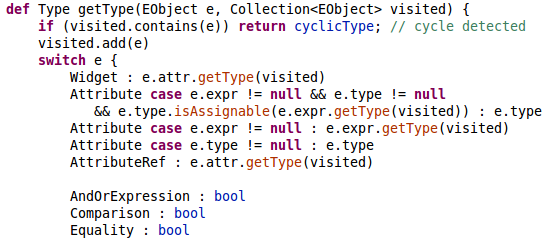
\includegraphics[width=\linewidth]{img/plain-xtext-provider.png}


\end{frame}